% !TeX program = xelatex
% !TeX encoding = UTF-8
% !TeX TXS-program:compile = txs:///xelatex | txs:///xelatex
\documentclass[aspectratio=169, table, 12pt]{beamer}

% Preamble bersama seluruh slide mata kuliah ini.
% Dipanggil dari slides/sessionXX/sessionXX.tex tepat sesudah baris
% \documentclass[aspectratio=169, table, 12pt]{beamer}
% Paket tambahan yang hanya dibutuhkan satu sesi ditulis di berkas sesi itu.

\usepackage{colortbl}
\usepackage{xcolor}
\usepackage{listings}
\usepackage{tabularx}
\usepackage{booktabs}
\usepackage{tikz}
\usepackage{pgfplots}
\usepackage{fontspec}
\usepackage[english,bahasai]{babel}
\pgfplotsset{compat=1.18}
\usetikzlibrary{arrows.meta, positioning, calc, fit, shapes.geometric,
  shapes.multipart, backgrounds, matrix, chains, trees}

\makeatletter
\def\input@path{{../theme/}}
\makeatother
\graphicspath{{../theme/}{../../figures/}}
% Stub symlink Windows memakai tema cadangan sampai aset institusi tersedia.
\IfFileExists{../theme/beamerthemePradita.sty}{%
  \usetheme{Pradita}
}{%
  \usetheme{Madrid}
  \setmainfont{TeX Gyre Heros}
  \setsansfont{TeX Gyre Heros}
  \setbeamertemplate{navigation symbols}{}
}

\definecolor{praditagreen}{RGB}{37, 113, 71}
\setbeamercolor{structure}{fg=praditagreen}
\setbeamercolor{palette primary}{bg=praditagreen,fg=white}
\setbeamercolor{palette secondary}{bg=praditagreen!80!black,fg=white}
\setbeamercolor{palette tertiary}{bg=praditagreen!60!black,fg=white}
\setbeamerfont{frametitle}{size=\large}
\setbeamertemplate{caption}[numbered]

% Ukuran header mengikuti teks agar judul panjang tidak menabrak logo.
\setbeamercolor{frametitle}{bg=white,fg=black}
\setbeamertemplate{frametitle}{%
  \begin{beamercolorbox}[wd=\paperwidth,sep=0.2cm]{frametitle}
    \begin{minipage}[c]{0.77\paperwidth}
      \raggedright\fontsize{16}{18}\selectfont\bfseries\insertframetitle
      \ifx\insertframesubtitle\empty\else
        \par\small\mdseries\insertframesubtitle
      \fi
    \end{minipage}\hfill
    \begin{minipage}[c]{0.15\paperwidth}
      \IfFileExists{../theme/classFiles/logo_universitas.png}{%
        
\includegraphics[width=\linewidth]{../theme/classFiles/logo_universitas.png}%
      }{}
    \end{minipage}
  \end{beamercolorbox}
}
\setbeamertemplate{footline}{%
  \ifnum\value{framenumber}>1
    \begin{beamercolorbox}[wd=\paperwidth,ht=0.35cm,dp=0.15cm,
      leftskip=0.3cm,rightskip=0.3cm]{palette primary}
      \footnotesize\bfseries\insertframenumber/\inserttotalframenumber
      \hfill IT40813
    \end{beamercolorbox}
  \fi
}
\DeclareRobustCommand{\berkas}[1]{\path{#1}}

% Tema membuat garis tabel berwarna putih. Dikembalikan agar tabel terbaca.
\arrayrulecolor{black}
\setlength{\arrayrulewidth}{0.5pt}

\lstdefinelanguage{yaml}{
  basicstyle=\ttfamily\scriptsize,
  keywordstyle=\color{blue}\bfseries,
  commentstyle=\color{gray}\itshape,
  stringstyle=\color{red},
  showstringspaces=false,
  breaklines=true,
  frame=lines,
  numbers=none,
  backgroundcolor=\color{lightgray!10},
  tabsize=2,
  morecomment=[l]{\#}
}

\lstdefinelanguage{json}{
  basicstyle=\ttfamily\scriptsize,
  stringstyle=\color{red},
  commentstyle=\color{gray},
  breaklines=true,
  showstringspaces=false,
  tabsize=2,
  numbers=none,
  frame=lines,
  backgroundcolor=\color{lightgray!10},
  string=[s]{"}{"}
}

\lstdefinelanguage{bash}{
  keywords={},
  basicstyle=\ttfamily\scriptsize,
  ndkeywords={docker, kubectl, helm, curl, git, terraform},
  ndkeywordstyle=\color{purple}\bfseries,
  sensitive=true,
  commentstyle=\color{gray},
  numbers=none,
  breaklines=true,
  frame=lines,
  backgroundcolor=\color{lightgray!10},
  tabsize=2,
  comment=[l]{\#},
  showstringspaces=false
}

\lstdefinelanguage{http}{
  keywords={GET, POST, PUT, PATCH, DELETE, HEAD, OPTIONS, HTTP},
  basicstyle=\ttfamily\scriptsize,
  keywordstyle=\color{blue}\bfseries,
  sensitive=true,
  numbers=none,
  breaklines=true,
  frame=lines,
  backgroundcolor=\color{lightgray!10},
  tabsize=2,
  showstringspaces=false
}

\subtitle{IT40813 · IT Governance, Risk \& Compliance}
\author{\textbf{Alfa Yohannis}}


% Sampul membatasi judul di panel putih tema rujukan Pradita.
\setbeamertemplate{title page}{%
  \begin{tikzpicture}[remember picture,overlay]
    \node[anchor=north west,inner sep=0pt,text width=8.8cm]
      at ([xshift=1cm,yshift=-3.15cm]current page.north west) {%
        {\small\insertsubtitle\par}\vspace{0.25cm}
        \resizebox{8.8cm}{!}{\begin{minipage}{12cm}
          \raggedright\color{praditagreen}\bfseries\inserttitle
        \end{minipage}}
      };
    \node[anchor=south west,inner sep=0pt]
      at ([xshift=1cm,yshift=1.65cm]current page.south west)
      {\small\insertdate};
    \node[anchor=west,inner sep=0pt,text=white]
      at ([xshift=0.8cm,yshift=0.75cm]current page.south west)
      {\small\insertauthor};
  \end{tikzpicture}
}


\title{\Huge Keamanan Informasi\\ \vspace{10pt} ISO/IEC 27001 dan NIST CSF}
\date{Pertemuan 06}

\begin{document}

\frame{\titlepage}

\begin{frame}
  \frametitle{Isi Pertemuan}
  \vspace{14pt}
  \begin{columns}[t]
    \column{0.5\textwidth}
    {\small\tableofcontents[sections={1-4}]}

    \column{0.5\textwidth}
    {\small\tableofcontents[sections={5-8}]}
  \end{columns}
\end{frame}

\begin{frame}{\hfill}
  \centering
  \Huge{\textbf{Kebijakan sudah ditandatangani.\\Mengapa 12 dari 120 akun\\masih luput?}}
\end{frame}

\section{Tujuan dan Konteks}

\begin{frame}{{\Large Tujuan Pembelajaran}}
  \vspace{10pt}
  \begin{itemize}
    \item Menjelaskan struktur ISMS (\textit{Information Security Management System}) menurut
          ISO/IEC 27001:2022 serta peran kontrol Annex A dan ISO/IEC 27002.
    \item Menyusun profil saat ini NIST CSF 2.0 untuk sebuah organisasi.
    \item Menganalisis celah kontrol keamanan dan mengaitkannya dengan skenario di \textit{risk
          register}.
  \end{itemize}
\end{frame}

\begin{frame}{{\Large Masalah: Kebijakan Ada, Akses Tetap Lemah}}
  \vspace{6pt}
  \small
  \begin{itemize}
    \item Pengandaian bab sebelumnya: 6 dari 30 akun sampel masih aktif setelah penugasan
          berakhir.
    \item Peninjauan berikutnya mencabut 24 dari 120 akun. Daftar peninjau hanya memuat 108 akun,
          sehingga 12 akun luput.
    \item Lima rumah sakit menjalankan SIMRS dengan versi berbeda. Bukti satu lokasi tidak mewakili
          seluruh Medikara.
    \item Kebijakan menunjukkan niat. Hasil peninjauan membuktikan pelaksanaan.
    \item Hasil kerja: profil saat ini dan daftar celah untuk tonggak C2.
  \end{itemize}
\end{frame}

\begin{frame}{{\Large Diagram Konsep Bab 6}}
  \centering
  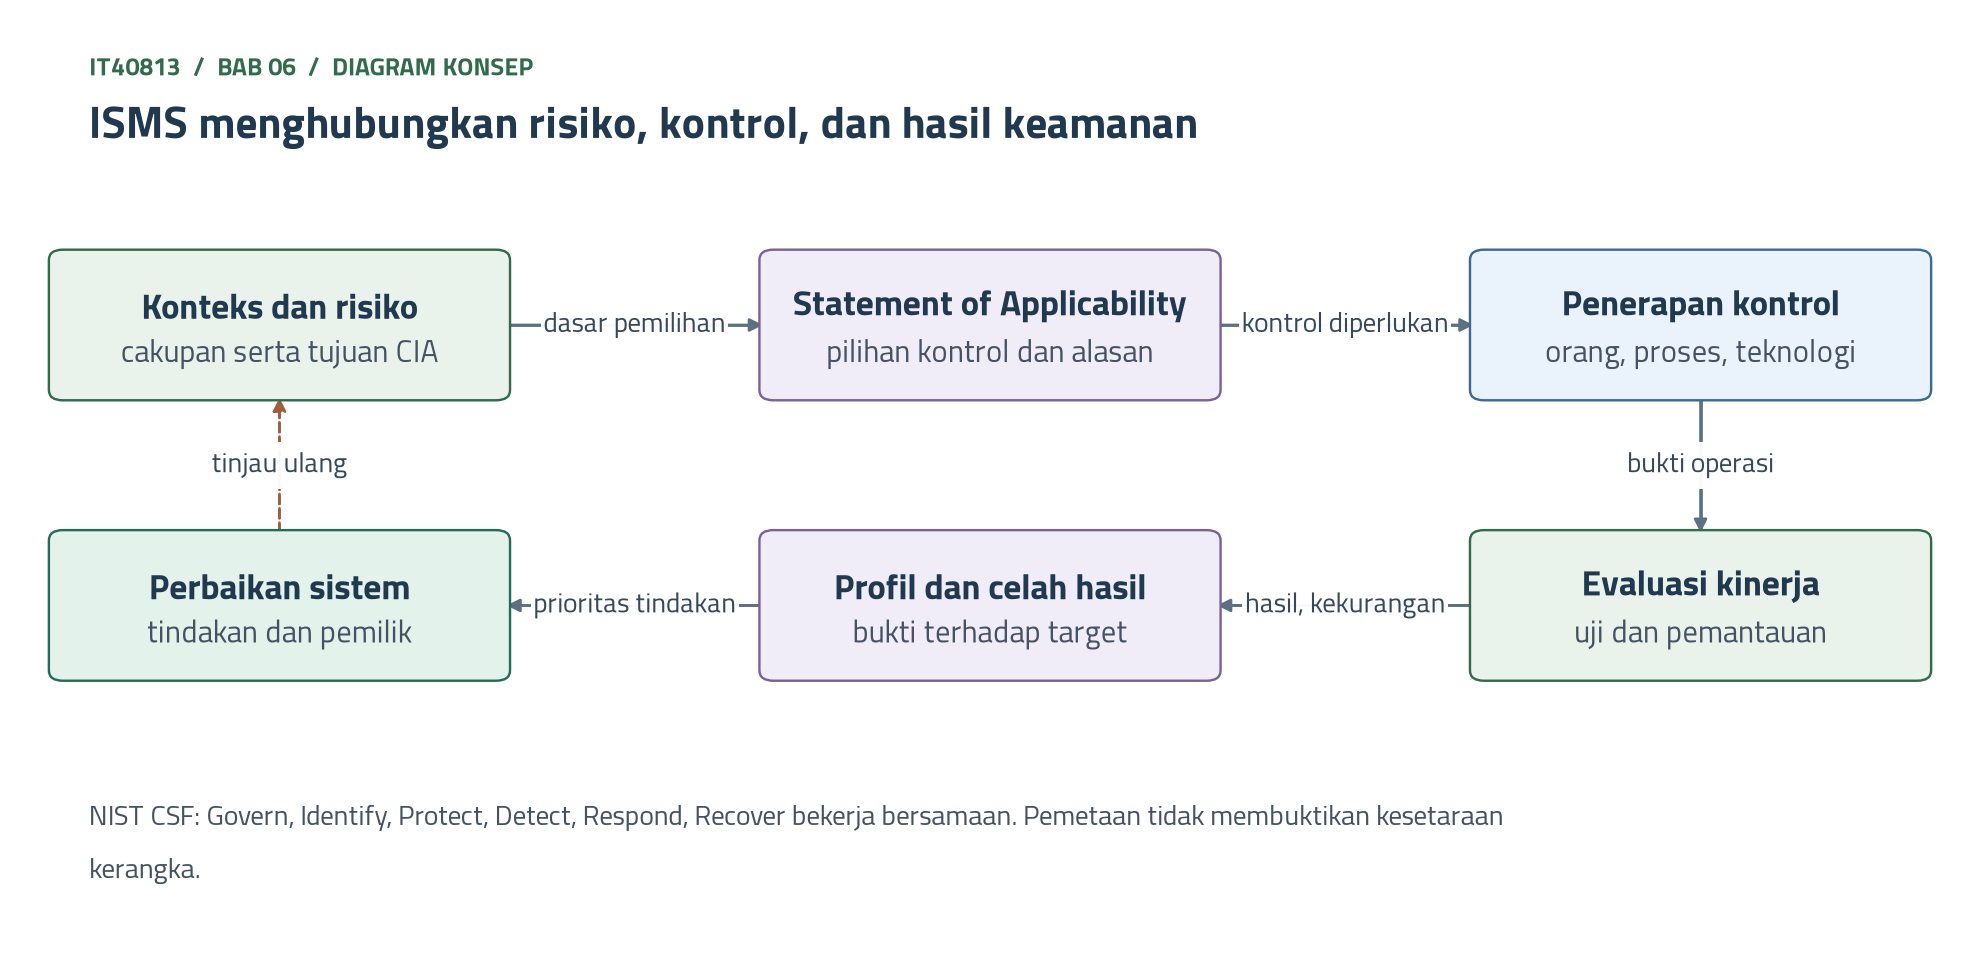
\includegraphics[width=0.96\textwidth,height=0.77\textheight,keepaspectratio]{../../figures/ch06-diagram-konsep.png}
  \label{fig:session06-ilustrasi-bab}
\end{frame}

\section{Tiga Tujuan Pelindungan}

\begin{frame}{{\Large Kerahasiaan, Integritas, dan Ketersediaan}}
  \vspace{4pt}
  \footnotesize
  \begin{tabularx}{\textwidth}{|>{\raggedright\arraybackslash}p{0.2\textwidth}|>{\raggedright\arraybackslash}X|>{\raggedright\arraybackslash}X|>{\raggedright\arraybackslash}p{0.1\textwidth}|}
    \hline
    \textbf{Tujuan} & \textbf{Pertanyaan} & \textbf{Bukti contoh} & \textbf{Risiko} \\ \hline
    Kerahasiaan & Apakah vendor hanya melihat data penugasannya? & Persetujuan dan pembatasan
    akses & R-01 \\ \hline
    Integritas & Siapa mengubah alergi dan kapan? & Jejak perubahan yang terlindungi & R-02 \\
    \hline
    Ketersediaan & Apakah data dapat dibaca saat gangguan? & Hasil uji pemulihan dan akses darurat
    & R-05 \\ \hline
  \end{tabularx}

  \vspace{8pt}
  \small Analogi lemari obat: lemari terkunci mengurangi akses tidak sah, pencatatan keluar masuk
  menjaga ketepatan stok, dan kunci cadangan menjaga layanan. Konflik antartujuan diselesaikan
  sesuai konteks layanan.
\end{frame}

\begin{frame}{{\Large Dua Contoh: Bukan Hanya Kerahasiaan}}
  \vspace{6pt}
  \small
  \begin{itemize}
    \item Misalkan satu akun bersama dipakai 12 petugas sebuah bangsal.
    \item Dalam sebulan tercatat 40 perubahan riwayat alergi, dan tidak satu pun dapat ditelusuri
          kepada petugas tertentu. Kelemahannya integritas, R-02.
    \item Misalkan semua akses darurat diblokir saat pengelola identitas terganggu 2 jam.
    \item Data terlindung, tetapi gangguan 2 jam menyentuh sekitar 548 kunjungan.
    \item Akses darurat yang terbatas, beralasan, dan ditinjau perlu diuji.
  \end{itemize}
\end{frame}

\begin{frame}{{\Large Membaca Penelitian: WannaCry pada NHS}}
  \vspace{6pt}
  \small
  \begin{itemize}
    \item Ghafur dan rekan (2019) menelaah serangan 2017 dengan data episode rumah sakit.
    \item 34 \textit{trust} terinfeksi; sekitar 13.500 janji rawat jalan dibatalkan pada pekan
          serangan.
    \item Pendaftaran gawat darurat turun sekitar 4 persen, elektif sekitar 9 persen, per hari per
          rumah sakit.
    \item Kerugian kegiatan £5,9 juta. Kematian tidak naik, tetapi disebut ukuran kasar bahaya bagi
          pasien.
    \item Angka ini tidak disalin ke Medikara. Yang dipelajari adalah cara mengukurnya.
  \end{itemize}
\end{frame}

\section{Sistem Manajemen}

\begin{frame}{{\Large ISMS: Sistem, Bukan Daftar Alat}}
  \vspace{6pt}
  \small
  \begin{itemize}
    \item ISMS menghubungkan kebijakan, risiko, pelaksanaan, evaluasi, dan perbaikan.
    \item ISO/IEC 27001 menetapkan persyaratannya pada klausul 4 sampai 10.
    \item Analogi dapur: cairan pembersih belum memastikan dapur bersih. Jadwal, pelaksana,
          pemeriksaan, dan peninjauan membentuk sistem.
    \item Amandemen 1:2024 hanya mengubah 4.1 dan 4.2: apakah perubahan iklim isu yang relevan.
    \item Naskah ISO berbayar. Rincian klausul perlu dicocokkan ke naskah berlisensi.
  \end{itemize}
\end{frame}

\begin{frame}{{\Large Klausul 4 sampai 10 sebagai Satu Sistem}}
  \vspace{6pt}
  \begin{center}
    \resizebox{0.95\textwidth}{!}{\begin{tikzpicture}[
  font=\scriptsize,
  tahap/.style={draw, rounded corners, align=center, text width=2.35cm,
    minimum height=1.25cm, fill=blue!8},
  panah/.style={-{Stealth[length=2mm]}, thick}]
  \node[tahap, fill=praditagreen!15] (k4) at (0,0)
    {\textbf{Klausul 4}\\Konteks\\{\tiny\mdseries cakupan dan pihak terkait}};
  \node[tahap] (k5) at (3.05,0)
    {\textbf{Klausul 5}\\Kepemimpinan\\{\tiny\mdseries kebijakan dan peran}};
  \node[tahap] (k6) at (6.1,0)
    {\textbf{Klausul 6}\\Perencanaan\\{\tiny\mdseries risiko, SoA, sasaran}};
  \node[tahap] (k7) at (9.15,0)
    {\textbf{Klausul 7}\\Dukungan\\{\tiny\mdseries orang dan dokumen}};
  \node[tahap] (k8) at (9.15,-2.0)
    {\textbf{Klausul 8}\\Operasi\\{\tiny\mdseries kontrol dijalankan}};
  \node[tahap, fill=orange!12] (k9) at (6.1,-2.0)
    {\textbf{Klausul 9}\\Evaluasi kinerja\\{\tiny\mdseries uji, audit, tinjauan}};
  \node[tahap, fill=green!10] (k10) at (3.05,-2.0)
    {\textbf{Klausul 10}\\Perbaikan\\{\tiny\mdseries koreksi yang diverifikasi}};
  \draw[panah] (k4) -- (k5);
  \draw[panah] (k5) -- (k6);
  \draw[panah] (k6) -- (k7);
  \draw[panah] (k7) -- (k8);
  \draw[panah] (k8) -- (k9);
  \draw[panah] (k9) -- (k10);
  \draw[panah, dashed] (k10.west) -| node[pos=0.75, left, align=right]
    {tinjau\\ulang} (k4.south);
\end{tikzpicture}
}
  \end{center}
  \small Ringkasan pembelajaran, bukan reproduksi isi standar. SoA adalah \textit{Statement of
  Applicability}.
\end{frame}

\begin{frame}{{\Large Klausul pada Kontrol AC-01 (Misalkan)}}
  \vspace{2pt}
  \scriptsize
  \begin{tabularx}{\textwidth}{|>{\raggedright\arraybackslash}p{0.22\textwidth}|>{\raggedright\arraybackslash}X|>{\raggedright\arraybackslash}X|}
    \hline
    \textbf{Klausul} & \textbf{Pertanyaan} & \textbf{Bukti pada AC-01} \\ \hline
    4 Konteks & Sistem, lokasi, dan pihak mana yang masuk cakupan? & 5 rumah sakit, Medikara+, 120
    akun; K-01 \\ \hline
    5 Kepemimpinan & Siapa menetapkan kebijakan dan peran? & Kebijakan akses; direksi menerima
    risiko sisa R-01 \\ \hline
    6 Perencanaan & Risiko dan kontrol apa yang dipilih? & R-01 skor $3 \times 4 = 12$; baris SoA;
    nol akun tanpa pemilik \\ \hline
    7 Dukungan & Apakah orang dan dokumen cukup? & Peninjau ditunjuk; prosedur tertulis \\ \hline
    8 Operasi & Apakah kontrol dijalankan? & Daftar akun, penandaan, tiket pencabutan \\ \hline
    9 Evaluasi kinerja & Apakah kontrol bekerja? & 108 dari 120 akun; audit 6 dari 30; tinjauan
    pimpinan \\ \hline
    10 Perbaikan & Apa yang berubah karena temuan? & Prosedur keluar vendor diubah; diuji ulang \\
    \hline
  \end{tabularx}
\end{frame}

\begin{frame}{{\Large Dua Contoh: Kegiatan dan Sistem}}
  \vspace{6pt}
  \small
  \begin{itemize}
    \item Misalkan alat pemantauan menghasilkan 300 alarm per bulan pada tiap 5 rumah sakit, total
          1.500.
    \item Dengan 10 menit per alarm, kerjanya 250 jam per bulan, lebih dari satu orang penuh waktu.
    \item Misalkan AC-01 bulan pertama mencabut 24 dari 120 akun. Sebabnya: tanggal berakhir
          penugasan tidak masuk daftar.
    \item Setelah prosedur diubah, pencabutan turun menjadi 9, 5, dan 2 akun, atau sekitar 92 persen.
    \item Temuan 12 akun tidak selesai hanya dengan mencabut 12 akun.
  \end{itemize}
\end{frame}

\begin{frame}{{\Large Sertifikat dan Ruang Lingkup}}
  \vspace{6pt}
  \small
  \begin{itemize}
    \item Misalkan sertifikat hanya untuk pusat data: 36 fasilitas layanan berada di luar lingkupnya.
    \item Misalkan sertifikat vendor berlaku 14 bulan, tetapi lingkupnya hanya pengembangan aplikasi.
          Akun dukungan tidak tercakup.
    \item Periksa tanggal, penerbit, ruang lingkup, dan temuan.
    \item Culot dan rekan (2021) mengelompokkan penelitian ke lima fokus: standar lain, motivasi,
          masalah penerapan, hasil, dan konteks.
    \item Pakai lima fokus itu sebagai daftar pertanyaan atas klaim ``sudah bersertifikat''.
  \end{itemize}
\end{frame}

\section{Annex A dan SoA}

\begin{frame}{{\Large Annex A: 93 Kontrol dalam Empat Tema}}
  \vspace{2pt}
  \footnotesize
  \begin{tabularx}{\textwidth}{|>{\raggedright\arraybackslash}p{0.09\textwidth}|>{\raggedright\arraybackslash}p{0.17\textwidth}|>{\raggedright\arraybackslash}p{0.09\textwidth}|>{\raggedright\arraybackslash}X|}
    \hline
    \textbf{Nomor} & \textbf{Tema} & \textbf{Jumlah} & \textbf{Contoh topik pada Medikara} \\ \hline
    5 & Organisasi & 37 & 5.18 hak akses; 5.19 dan 5.20 pemasok; 5.26 tanggapan insiden \\ \hline
    6 & Manusia & 8 & Pelatihan petugas; tanggung jawab setelah penugasan berakhir \\ \hline
    7 & Fisik & 14 & Ruang server dan perangkat di 36 fasilitas \\ \hline
    8 & Teknologi & 34 & 8.5 autentikasi; 8.13 cadangan; 8.15 pencatatan; 8.16 pemantauan \\ \hline
    Total & & 93 & \\ \hline
  \end{tabularx}

  \vspace{8pt}
  \small Annex A dipakai untuk memeriksa bahwa tidak ada kontrol perlu yang terlewat, bukan sebagai
  daftar yang otomatis wajib. Uraian topik bukan terjemahan resmi.
\end{frame}

\begin{frame}{{\Large Persyaratan dan Panduan}}
  \vspace{2pt}
  \footnotesize
  \begin{tabularx}{\textwidth}{|>{\raggedright\arraybackslash}p{0.22\textwidth}|>{\raggedright\arraybackslash}p{0.24\textwidth}|>{\raggedright\arraybackslash}X|}
    \hline
    \textbf{Standar} & \textbf{Sifat} & \textbf{Pemakaian pada Medikara} \\ \hline
    ISO/IEC 27001:2022 & Persyaratan sistem manajemen & Menilai ruang lingkup ISMS, SoA, evaluasi,
    dan perbaikan \\ \hline
    ISO/IEC 27002:2022 & Panduan penerapan kontrol & Cara merancang peninjauan hak akses pada AC-01
    \\ \hline
    ISO 27799:2025 & Panduan kontrol untuk organisasi kesehatan & Rekam medis elektronik, perangkat
    digital fasilitas, telekonsultasi Medikara+ \\ \hline
  \end{tabularx}

  \vspace{8pt}
  \small Sertifikasi mengacu pada persyaratan, bukan panduan. Pembatasan akses tidak boleh merusak
  kebutuhan pelayanan darurat. Bab 5 membatasi pengecualian darurat akun vendor paling lama 24 jam.
\end{frame}

\begin{frame}{{\Large Dari Risiko ke SoA}}
  \vspace{6pt}
  \begin{center}
    \resizebox{0.95\textwidth}{!}{\begin{tikzpicture}[
  font=\scriptsize,
  tahap/.style={draw, rounded corners, align=center, text width=3.0cm,
    minimum height=1.1cm, fill=blue!8},
  panah/.style={-{Stealth[length=2mm]}, thick}]
  \node[tahap, fill=praditagreen!15] (risiko) at (0,0)
    {\textbf{Risiko R-01}\\{\tiny\mdseries skor $3 \times 4 = 12$, dinilai pada Bab 5}};
  \node[tahap] (tangani) at (4.1,0)
    {\textbf{Penanganan dipilih}\\{\tiny\mdseries kurangi paparan akun vendor}};
  \node[tahap] (perlu) at (8.2,0)
    {\textbf{Kontrol diperlukan}\\{\tiny\mdseries AC-01 dan pemantauan aktivitas}};
  \node[tahap] (banding) at (8.2,-1.9)
    {\textbf{Dibandingkan dengan Annex A}\\{\tiny\mdseries 93 kontrol sebagai rujukan}};
  \node[tahap, fill=orange!12] (soa) at (4.1,-1.9)
    {\textbf{SoA}\\{\tiny\mdseries kontrol, alasan, status, pengecualian}};
  \node[tahap, fill=green!10] (bukti) at (0,-1.9)
    {\textbf{Bukti operasi}\\{\tiny\mdseries daftar akun, keputusan, tiket pencabutan}};
  \draw[panah] (risiko) -- (tangani);
  \draw[panah] (tangani) -- (perlu);
  \draw[panah] (perlu) -- (banding);
  \draw[panah] (banding) -- (soa);
  \draw[panah] (soa) -- (bukti);
  \draw[panah, dashed] (bukti) -- node[right, align=left] {tinjau ulang} (risiko);
\end{tikzpicture}
}
  \end{center}
  \small SoA memuat kontrol yang diperlukan, alasan, status penerapan, dan alasan pengecualian.
  Analogi perjalanan: perlengkapan yang tidak dibawa tetap dinilai terhadap tujuan.
\end{frame}

\begin{frame}{{\Large Penalaran SoA}}
  \vspace{2pt}
  \scriptsize
  \begin{tabularx}{\textwidth}{|>{\raggedright\arraybackslash}p{0.27\textwidth}|>{\raggedright\arraybackslash}X|>{\raggedright\arraybackslash}X|}
    \hline
    \textbf{Kontrol} & \textbf{Alasan} & \textbf{Status dan bukti} \\ \hline
    AC-01 peninjauan hak akses (5.18) & Akses vendor berlebih pada R-01; K-01 & Sebagian; bukti 1 dari
    5 rumah sakit \\ \hline
    Pencatatan aktivitas (8.15) & Menelusuri perubahan data pada R-01, R-02 & Catatan ada; tinjauan
    belum terbukti \\ \hline
    Cadangan dan pemulihan (8.13) & Menjaga data saat gangguan pada R-05; K-02 & Cadangan ada; uji
    pemulihan diminta \\ \hline
    Pengembangan alih daya (8.30) & Vendor mengubah Medikara+; R-07 & Usulan pengecualian ditolak \\
    \hline
  \end{tabularx}

  \vspace{8pt}
  \small Kode sering tertukar: AC-01 adalah kode lokal Medikara, 5.18 nomor Annex A, dan AC-01 pada
  berkas NIST milik SP 800-53. Tulis selalu sumber kodenya.
\end{frame}

\begin{frame}{{\Large Kasus Medikara: SoA untuk Cakupan Terbatas}}
  \vspace{6pt}
  \small
  \begin{itemize}
    \item Misalkan 93 kontrol dinilai untuk 5 rumah sakit dan Medikara+.
    \item Hasil awal: 84 diperlukan dan 9 diusulkan dikecualikan, sekitar 9,7 persen.
    \item Tiga usulan ditolak karena R-07 menunjukkan vendor tetap mengubah Medikara+.
    \item Hasil akhir: 87 diperlukan dan 6 dikecualikan, dengan alasan, penyetuju, dan tanggal tinjau
          ulang.
    \item Jumlah kontrol bukan ukuran keamanan. Kualitas alasannya yang dinilai.
  \end{itemize}
\end{frame}

\section{Enam Fungsi CSF}

\begin{frame}{{\Large Struktur Inti NIST CSF 2.0}}
  \vspace{6pt}
  \small
  \begin{itemize}
    \item Hierarki hasil: 6 fungsi, 22 kategori, dan 106 subkategori.
    \item Hasil itu bukan daftar periksa tindakan, dan urutannya bukan urutan kerja.
    \item CSF menjelaskan hasil yang diinginkan tanpa menetapkan cara mencapainya.
    \item Analogi gedung: pintu yang kuat tidak menggantikan petugas dan rencana penanganan.
    \item Layanan API dan cloud masuk cakupan profil. Rinciannya pada IT40613 dan IT40713.
  \end{itemize}
\end{frame}

\begin{frame}{{\Large Govern Mengarahkan Lima Fungsi Lain}}
  \begin{center}
    \resizebox{!}{5.6cm}{\begin{tikzpicture}[
  font=\scriptsize,
  fungsi/.style={draw, rounded corners, align=center, text width=2.2cm,
    minimum height=0.95cm, fill=blue!8},
  panah/.style={-{Stealth[length=2mm]}, thick}]
  \node[fungsi, fill=praditagreen!15, text width=2.7cm, minimum height=1.2cm] (gv) at (0,0)
    {\textbf{Govern}\\{\tiny\mdseries arah, peran, kebijakan, pengawasan, pemasok}};
  \node[fungsi] (id) at (0,2.3) {\textbf{Identify}\\{\tiny\mdseries aset, risiko, perbaikan}};
  \node[fungsi] (pr) at (4.2,0.8) {\textbf{Protect}\\{\tiny\mdseries akses, data, platform}};
  \node[fungsi] (de) at (2.55,-2.0) {\textbf{Detect}\\{\tiny\mdseries pemantauan, analisis}};
  \node[fungsi] (rs) at (-2.55,-2.0) {\textbf{Respond}\\{\tiny\mdseries insiden, komunikasi}};
  \node[fungsi] (rc) at (-4.2,0.8) {\textbf{Recover}\\{\tiny\mdseries pemulihan, komunikasi}};
  \draw[gray, thin] (id) -- (pr) -- (de) -- (rs) -- (rc) -- (id);
  \draw[panah] (gv) -- (id);
  \draw[panah] (gv) -- (pr);
  \draw[panah] (gv) -- (de);
  \draw[panah] (gv) -- (rs);
  \draw[panah] (gv) -- (rc);
\end{tikzpicture}
}
  \end{center}
\end{frame}

\begin{frame}{{\Large Hasil dan Pertanyaan pada Enam Fungsi}}
  \vspace{2pt}
  \scriptsize
  \begin{tabularx}{\textwidth}{|>{\raggedright\arraybackslash}p{0.13\textwidth}|>{\raggedright\arraybackslash}X|>{\raggedright\arraybackslash}X|>{\raggedright\arraybackslash}p{0.24\textwidth}|}
    \hline
    \textbf{Fungsi} & \textbf{Hasil (ringkasan)} & \textbf{Pertanyaan Medikara} & \textbf{Bukti contoh}
    \\ \hline
    Govern & Strategi, harapan, dan kebijakan risiko ditetapkan serta dipantau & Siapa menerima
    risiko akses vendor? & Keputusan dan wewenang \\ \hline
    Identify & Risiko keamanan saat ini dipahami & Sistem dan data apa yang terlibat? & Inventaris,
    alur data \\ \hline
    Protect & Pengaman dipakai untuk mengelola risiko & Bagaimana akses dibatasi? & Daftar hak, bukti
    AC-01 \\ \hline
    Detect & Kemungkinan serangan ditemukan dan dianalisis & Bagaimana akses menyimpang diketahui? &
    Catatan alarm dan tinjauan \\ \hline
    Respond & Tindakan atas insiden yang terdeteksi diambil & Siapa membekukan akses? & Prosedur,
    hasil latihan \\ \hline
    Recover & Aset dan operasi yang terdampak dipulihkan & Bagaimana data dipulihkan? & Hasil uji
    pemulihan \\ \hline
  \end{tabularx}
\end{frame}

\begin{frame}{{\Large Dua Contoh: Fungsi Saling Melengkapi}}
  \vspace{6pt}
  \small
  \begin{itemize}
    \item Misalkan seluruh 108 akun pada daftar peninjau memakai MFA. Cakupannya tampak 100 persen.
    \item Terhadap populasi 120 akun, cakupannya hanya 90 persen. Protect tidak menolong bila
          Identify belum lengkap.
    \item Misalkan alarm akses diterima dalam 5 menit, tetapi tidak ada yang berwenang membekukan
          akun.
    \item Data latihan Bab 1: akun dukungan memanggil data 8 malam dan baru diketahui pada hari ke-11.
    \item Kecepatan deteksi belum menghasilkan penanganan.
  \end{itemize}
\end{frame}

\begin{frame}{{\Large Mengapa Govern Ditambahkan}}
  \vspace{2pt}
  \scriptsize
  \begin{tabularx}{\textwidth}{|>{\raggedright\arraybackslash}p{0.14\textwidth}|>{\raggedright\arraybackslash}X|>{\raggedright\arraybackslash}X|}
    \hline
    \textbf{Subkategori} & \textbf{Hasil (ringkasan)} & \textbf{Hasil kerja Medikara} \\ \hline
    GV.OC-03 & Persyaratan hukum, regulasi, dan kontrak dipahami serta dikelola & Register K-01
    sampai K-16, Bab 3 \\ \hline
    GV.RM-02 & Pernyataan \textit{risk appetite} dan \textit{risk tolerance} ditetapkan & Nol akun
    vendor aktif tanpa pemilik, Bab 5 \\ \hline
    GV.RR-02 & Peran, tanggung jawab, dan wewenang ditegakkan & Hak keputusan akses vendor, Bab 2 \\
    \hline
    GV.SC-07 & Risiko pemasok dipahami dan dipantau sepanjang hubungan & Vendor Medikara+, R-01,
    insiden 2025 \\ \hline
  \end{tabularx}

  \vspace{8pt}
  \small Versi 1.1 punya lima fungsi. Versi 2.0 menambahkan Govern dan menonjolkan tata kelola serta
  rantai pasok. Tanpa Govern, penilaian mudah berhenti sebagai urusan tim teknis (penafsiran bab).
\end{frame}

\begin{frame}{{\Large ISO/IEC 27001 dan NIST CSF}}
  \vspace{2pt}
  \scriptsize
  \begin{tabularx}{\textwidth}{|>{\raggedright\arraybackslash}p{0.17\textwidth}|>{\raggedright\arraybackslash}X|>{\raggedright\arraybackslash}X|}
    \hline
    \textbf{Pembeda} & \textbf{ISO/IEC 27001:2022} & \textbf{NIST CSF 2.0} \\ \hline
    Sifat & Persyaratan sistem manajemen & Taksonomi hasil, tanpa menetapkan cara \\ \hline
    Unsur & Klausul 4 sampai 10, 93 kontrol Annex A, SoA & 6 fungsi, 22 kategori, 106 subkategori,
    profil, \textit{tier} \\ \hline
    Pemeriksaan & Dapat disertifikasi dalam ruang lingkup & Tidak ada skema sertifikasi pada naskah
    2.0 \\ \hline
    Akses naskah & Berbayar & Terbuka \\ \hline
    Luaran Medikara & Ruang lingkup ISMS, SoA, hasil evaluasi & Profil saat ini, celah, profil target
    Bab 8 \\ \hline
  \end{tabularx}

  \vspace{8pt}
  \small Keduanya melengkapi, bukan menggantikan.
\end{frame}

\section{Profil dan Tier}

\begin{frame}{{\Large Lima Langkah Profil}}
  \vspace{6pt}
  \begin{center}
    \resizebox{0.95\textwidth}{!}{\begin{tikzpicture}[
  font=\scriptsize,
  tahap/.style={draw, rounded corners, align=center, text width=1.9cm,
    minimum height=1.0cm, fill=blue!8},
  hasil/.style={draw, align=center, text width=1.9cm, minimum height=1.05cm,
    fill=white, font=\tiny},
  panah/.style={-{Stealth[length=2mm]}, thick}]
  \node[tahap] (s1) at (0,0) {1. Tetapkan cakupan};
  \node[tahap] (s2) at (2.45,0) {2. Kumpulkan informasi};
  \node[tahap, fill=orange!12] (s3) at (4.9,0) {3. Buat profil};
  \node[tahap, fill=orange!12] (s4) at (7.35,0) {4. Analisis celah dan rencana};
  \node[tahap, fill=green!10] (s5) at (9.8,0) {5. Jalankan dan perbarui};
  \node[hasil] (h1) at (0,-1.55) {5 rumah sakit, Medikara+, 120 akun, 12 bulan};
  \node[hasil] (h2) at (2.45,-1.55) {Register Bab 3, register Bab 5, sumber bukti};
  \node[hasil] (h3) at (4.9,-1.55) {14 subkategori dengan status lokal};
  \node[hasil] (h4) at (7.35,-1.55) {6 celah, 3 prioritas untuk Bab 8};
  \node[hasil] (h5) at (9.8,-1.55) {Profil target Bab 8, tonggak C3};
  \draw[panah] (s1) -- (s2);
  \draw[panah] (s2) -- (s3);
  \draw[panah] (s3) -- (s4);
  \draw[panah] (s4) -- (s5);
  \foreach \nomor in {1,2,3,4,5} {
    \draw[gray, thin] (s\nomor) -- (h\nomor);
  }
  \draw[panah, dashed] (s5.north) -- ++(0,0.4) -| node[pos=0.25, above] {ulangi} (s1.north);
\end{tikzpicture}
}
  \end{center}
  \small Profil saat ini menyebut hasil yang sedang dicapai dan seberapa jauh. Bab 6 mengerjakan
  langkah 1 sampai 4. Profil target dirancang pada Bab 8.
\end{frame}

\begin{frame}{{\Large Status Lokal dan Batas Bukti}}
  \vspace{2pt}
  \scriptsize
  \begin{tabularx}{\textwidth}{|>{\raggedright\arraybackslash}p{0.2\textwidth}|>{\raggedright\arraybackslash}X|>{\raggedright\arraybackslash}X|}
    \hline
    \textbf{Status lokal} & \textbf{Arti} & \textbf{Tindakan} \\ \hline
    Terbukti & Bukti sesuai cakupan dan periode & Simpan sumber dan peninjau \\ \hline
    Sebagian & Sebagian hasil atau lokasi belum tercakup & Jelaskan celah spesifik \\ \hline
    Belum ada bukti & Klaim belum dapat diuji & Minta bukti; jangan beri status lulus \\ \hline
    Tidak relevan & Ada alasan terhadap cakupan & Catat persetujuan dan tinjau ulang \\ \hline
  \end{tabularx}

  \vspace{6pt}
  \small Audit: 24 dari 30 akun sesuai, atau 80 persen. Kesimpulannya ada 6 pengecualian dalam
  sampel, bukan 80 persen aman. Misalkan 150 cadangan berhasil dalam 30 hari pada 5 rumah sakit:
  pemulihan belum terbukti sebelum diuji.
\end{frame}

\begin{frame}{{\Large Profil: Govern dan Identify (Misalkan)}}
  \vspace{2pt}
  \footnotesize
  \begin{tabularx}{\textwidth}{|>{\raggedright\arraybackslash}p{0.14\textwidth}|>{\raggedright\arraybackslash}p{0.13\textwidth}|>{\raggedright\arraybackslash}X|>{\raggedright\arraybackslash}p{0.18\textwidth}|}
    \hline
    \textbf{Subkategori} & \textbf{Status} & \textbf{Bukti dan batasnya} & \textbf{Tautan} \\ \hline
    GV.OC-03 & Sebagian & Register 16 baris; 7 baris belum diverifikasi & K-01 sampai K-16 \\ \hline
    GV.RM-02 & Sebagian & Batas nol akun sudah dirumuskan; pemantauan belum teruji & R-01 \\ \hline
    GV.RR-02 & Sebagian & Hak keputusan tertulis; 12 akun belum punya pemilik & R-01 \\ \hline
    GV.SC-07 & Sebagian & Tinjauan berkala belum ada; laporan insiden telat & R-01, R-08, K-05 \\
    \hline
    ID.AM-02 & Sebagian & Daftar lokal 5 rumah sakit belum direkonsiliasi & R-02 \\ \hline
  \end{tabularx}
\end{frame}

\begin{frame}{{\Large Profil: Protect sampai Recover (Misalkan)}}
  \vspace{2pt}
  \scriptsize
  \begin{tabularx}{\textwidth}{|>{\raggedright\arraybackslash}p{0.13\textwidth}|>{\raggedright\arraybackslash}p{0.18\textwidth}|>{\raggedright\arraybackslash}X|>{\raggedright\arraybackslash}p{0.2\textwidth}|}
    \hline
    \textbf{Subkategori} & \textbf{Status} & \textbf{Bukti dan batasnya} & \textbf{Tautan} \\ \hline
    PR.AA-01 & Sebagian & Akun bersama ditemukan & R-02, K-01 \\ \hline
    PR.AA-03 & Sebagian & MFA pada 108 akun; 12 tidak diketahui & R-01, K-01 \\ \hline
    PR.AA-05 & Sebagian & Bukti AC-01 pada 1 dari 5 rumah sakit & R-01, R-02, K-01 \\ \hline
    PR.AA-06 & Tidak relevan & Vendor jarak jauh; tinjau bila hadir di lokasi & Tidak ada \\ \hline
    PR.PS-04 & Terbukti & Catatan pada 5 SIMRS selama 12 bulan & R-01 \\ \hline
    PR.DS-11 & Sebagian & Cadangan malam berjalan; uji belum ada & R-05, K-02 \\ \hline
    DE.CM-03 & Sebagian & Catatan ada; tinjauan belum ada & R-01, K-01 \\ \hline
    RS.MA-01 & Belum ada bukti & Prosedur belum dilatih bersama vendor & R-01, R-12, K-04, K-05 \\
    \hline
    RC.RP-03 & Belum ada bukti & Hasil verifikasi belum tersedia & R-05, K-02 \\ \hline
  \end{tabularx}

  \vspace{4pt}
  \small 14 dari 106 subkategori: 1 terbukti, 10 sebagian, 2 belum ada bukti, 1 tidak relevan.
\end{frame}

\begin{frame}{{\Large Tier Bukan Rata-Rata}}
  \vspace{2pt}
  \scriptsize
  \begin{tabularx}{\textwidth}{|>{\raggedright\arraybackslash}p{0.2\textwidth}|>{\raggedright\arraybackslash}X|>{\raggedright\arraybackslash}X|}
    \hline
    \textbf{Tier} & \textbf{Tata kelola risiko (ringkasan)} & \textbf{Risiko pemasok (ringkasan)} \\
    \hline
    Tier 1, Partial & Strategi risiko diterapkan seadanya & Umumnya tidak menyadari risiko pemasok \\
    \hline
    Tier 2, Risk Informed & Disetujui manajemen, mungkin belum menjadi kebijakan organisasi & Sadar,
    tetapi belum bertindak konsisten atau formal \\ \hline
    Tier 3, Repeatable & Disetujui resmi sebagai kebijakan, diperbarui berkala & Perjanjian tertulis
    dan pemantauan \\ \hline
    Tier 4, Adaptive & Dipantau pimpinan bersama risiko keuangan dan risiko lain & Informasi hampir
    waktu nyata \\ \hline
  \end{tabularx}

  \vspace{6pt}
  \small Pimpinan memilih \textit{tier} per organisasi, fungsi, atau kategori. Rumus nilai 4, 2, dan
  1 yang menghasilkan rata-rata 2,0 tidak berdasar. Status lokal, \textit{tier}, dan kapabilitas
  COBIT tidak saling dikonversi.
\end{frame}

\section{Celah Kontrol}

\begin{frame}{{\Large Pemetaan Menunjukkan Kontribusi}}
  \vspace{6pt}
  \small
  \begin{itemize}
    \item Hubungan subkategori, kontrol, risiko, dan kewajiban dapat banyak ke banyak.
    \item NIST SP 1347: NIST tidak menguji kebenaran pemetaan dari pihak lain.
    \item Berkas NIST memuat dua daftar untuk PR.AA-05: 11 kontrol dan 6 kontrol, irisannya 5.
    \item Misalkan AC-01 hanya punya 12 dari 60 catatan bulanan, atau 20 persen: celah cakupan.
    \item Misalkan 0 dari 260 catatan tinjauan mingguan tersedia: celah deteksi dan tindak lanjut.
  \end{itemize}
\end{frame}

\begin{frame}{{\Large Pemetaan Subkategori ke Annex A}}
  \vspace{2pt}
  \scriptsize
  \begin{tabularx}{\textwidth}{|>{\raggedright\arraybackslash}p{0.13\textwidth}|>{\raggedright\arraybackslash}p{0.24\textwidth}|>{\raggedright\arraybackslash}X|>{\raggedright\arraybackslash}p{0.21\textwidth}|}
    \hline
    \textbf{Subkategori} & \textbf{Annex A} & \textbf{Kontrol Medikara} & \textbf{Risiko, kewajiban}
    \\ \hline
    PR.AA-05 & 5.15, 5.18, 8.2, 8.3, 8.18 & AC-01 peninjauan akses & R-01, R-02, K-01 \\ \hline
    PR.AA-01 & 5.15, 5.16, 5.18, 8.2, 8.5 & Akun per orang & R-02, K-01 \\ \hline
    PR.AA-03 & 5.15, 5.16, 5.17, 5.18, 8.5 & MFA akun vendor & R-01, K-01 \\ \hline
    ID.AM-02 & 5.9 & Inventaris sistem & R-02 \\ \hline
    PR.PS-04 & 8.15, 8.17 & Pencatatan aktivitas & R-01, K-01 \\ \hline
    DE.CM-03 & 7.4, 8.16 & Tinjauan catatan & R-01, K-01 \\ \hline
    PR.DS-11 & 8.13 & Cadangan lokasi terpisah & R-05, K-02 \\ \hline
    RC.RP-03 & 8.13 & Uji pemulihan & R-05, K-02 \\ \hline
    RS.MA-01 & 5.26, 5.27, 5.28 & Insiden bersama vendor & R-01, R-12, K-04, K-05 \\ \hline
    GV.SC-07 & 5.19, 5.20, 5.22, 5.31 & Tinjauan vendor & R-01, R-08, K-05 \\ \hline
  \end{tabularx}
\end{frame}

\begin{frame}{{\Large Daftar Celah (Misalkan)}}
  \vspace{2pt}
  \scriptsize
  \begin{tabularx}{\textwidth}{|>{\raggedright\arraybackslash}p{0.07\textwidth}|>{\raggedright\arraybackslash}X|>{\raggedright\arraybackslash}p{0.16\textwidth}|>{\raggedright\arraybackslash}p{0.23\textwidth}|>{\raggedright\arraybackslash}X|}
    \hline
    \textbf{ID} & \textbf{Belum tercapai} & \textbf{Risiko} & \textbf{Pemilik risiko; tindakan} &
    \textbf{Bukti penerimaan} \\ \hline
    G-01 & Belum lintas lokasi; 12 akun luput & R-01, K-01 & Pemilik Medikara+; kepala operasi TI &
    120 dari 120 akun cocok \\ \hline
    G-02 & Catatan tidak ditinjau & R-01, K-01 & Pemilik Medikara+; fungsi keamanan & Alarm uji
    ditangani \\ \hline
    G-03 & Pemulihan belum diuji & R-05, K-02 & Pemilik layanan; kepala operasi TI & Hasil disahkan
    \\ \hline
    G-04 & Hak lokal beda; akun bersama & R-02, K-01 & Pemilik SIMRS; pemilik layanan & Peran baku 5
    rumah sakit \\ \hline
    G-05 & Vendor terlambat melapor & R-01, R-12, K-04, K-05 & Pemilik Medikara+; pengelola vendor &
    Laporan dalam 12 jam \\ \hline
    G-06 & Inventaris belum direkonsiliasi & R-02 & Pemilik SIMRS; kepala TI & Satu inventaris
    disetujui \\ \hline
  \end{tabularx}

  \vspace{4pt}
  \small Pembanding sementara: batas Bab 5, register Bab 3, dan SoA.
\end{frame}

\begin{frame}{{\Large Keterlacakan Tiga Celah Prioritas}}
  \begin{center}
    \resizebox{0.95\textwidth}{!}{\begin{tikzpicture}[
  font=\scriptsize,
  judul/.style={draw, align=center, text width=1.9cm, minimum height=0.6cm,
    fill=praditagreen!15},
  sel/.style={draw, rounded corners, align=center, text width=1.9cm,
    minimum height=1.05cm, fill=blue!8},
  panah/.style={-{Stealth[length=2mm]}, thick}]
  \node[judul] at (0,0) {\textbf{Subkategori}};
  \node[judul] at (2.45,0) {\textbf{Status lokal}};
  \node[judul] at (4.9,0) {\textbf{Celah}};
  \node[judul] at (7.35,0) {\textbf{Kontrol}};
  \node[judul] at (9.8,0) {\textbf{Risiko, kewajiban}};
  \node[sel] (a1) at (0,-1.0) {PR.AA-05};
  \node[sel, fill=gray!35] (a2) at (2.45,-1.0) {Sebagian};
  \node[sel, fill=orange!12] (a3) at (4.9,-1.0)
    {\textbf{G-01}\\{\tiny\mdseries peninjauan belum lintas lokasi}};
  \node[sel] (a4) at (7.35,-1.0) {AC-01\\{\tiny\mdseries Annex A 5.15, 5.18}};
  \node[sel, fill=green!10] (a5) at (9.8,-1.0) {R-01, K-01};
  \node[sel] (b1) at (0,-2.3) {RC.RP-03};
  \node[sel, fill=red!22] (b2) at (2.45,-2.3) {Belum ada bukti};
  \node[sel, fill=orange!12] (b3) at (4.9,-2.3)
    {\textbf{G-03}\\{\tiny\mdseries pemulihan belum diuji}};
  \node[sel] (b4) at (7.35,-2.3) {Uji pemulihan\\{\tiny\mdseries Annex A 8.13}};
  \node[sel, fill=green!10] (b5) at (9.8,-2.3) {R-05, K-02};
  \node[sel] (c1) at (0,-3.6) {RS.MA-01, GV.SC-07};
  \node[sel, fill=red!22] (c2) at (2.45,-3.6) {Belum ada bukti};
  \node[sel, fill=orange!12] (c3) at (4.9,-3.6)
    {\textbf{G-05}\\{\tiny\mdseries vendor terlambat\\melapor}};
  \node[sel] (c4) at (7.35,-3.6) {Insiden vendor\\{\tiny\mdseries Annex A 5.20, 5.26}};
  \node[sel, fill=green!10] (c5) at (9.8,-3.6) {R-01, R-12, K-04, K-05};
  \foreach \baris in {a,b,c} {
    \draw[panah] (\baris1) -- (\baris2);
    \draw[panah] (\baris2) -- (\baris3);
    \draw[panah] (\baris3) -- (\baris4);
    \draw[panah] (\baris4) -- (\baris5);
  }
\end{tikzpicture}
}
  \end{center}
\end{frame}

\begin{frame}{{\Large Kasus Medikara: Tiga Prioritas untuk Bab 8}}
  \vspace{6pt}
  \small
  \begin{itemize}
    \item Bab 5: R-11 keselamatan, R-01 insiden 2025 dan K-01, R-05 harapan kerugian terbesar.
    \item Tim memilih G-01, G-03, dan G-05. Varian uji kontrak Bab 3: vendor melapor setelah 30 jam.
    \item G-01: 120 akun dikali 6 menit, atau 144 jam per tahun; anggaran Rp60 juta pada Bab 5.
    \item G-03: 144 uji pemulihan dikali 3 jam, atau 432 jam per tahun.
    \item Total 576 jam, sekitar 3,6 bulan kerja dari 52 staf TI. Rincian kelangsungan menunggu
          Bab 10.
  \end{itemize}
\end{frame}

\section{Aktivitas, Ringkasan, dan Latihan}

\begin{frame}{{\Large Aktivitas: Peran dan Langkah}}
  \vspace{6pt}
  \small
  \begin{itemize}
    \item Analis teknologi memimpin. Pemilik konteks memastikan bukti ada. Analis regulasi menandai
          kewajiban. Analis risiko menjaga tautan ke Bab 5.
    \item Tetapkan cakupan, lalu pilih subkategori pada keenam fungsi.
    \item Untuk Medikara: akses SIMRS, akun vendor, pencatatan \textit{log}, dan cadangan data.
    \item Nilai status berdasarkan bukti, lalu terjemahkan menjadi celah terhadap Annex A.
    \item Hubungkan celah ke risiko dan kewajiban, lalu pilih tiga prioritas untuk Bab 8.
  \end{itemize}
\end{frame}

\begin{frame}{{\Large Aktivitas: Luaran, C2, dan Berkas}}
  \vspace{6pt}
  \small
  \begin{itemize}
    \item Luaran: profil saat ini, daftar celah, catatan SoA, dan tiga prioritas.
    \item Tonggak C2 Kondisi Saat Ini, ditinjau menjelang UTS.
    \item Rubrik: bukti 35 persen, status 25 persen, risiko 25 persen, batas kesimpulan 15 persen.
    \item Berkas di \berkas{sources/chapter06}: \texttt{profil-csf-saat-ini.csv},
          \texttt{contoh-profil-medikara.csv}, \texttt{celah-kontrol.csv},
          \texttt{pemetaan-csf-annex-a.csv}, \texttt{panduan-bukti.md}, \texttt{catatan-soa.md}.
    \item Data nyata wajib berizin dan dianonimkan. Pemeriksaan teknis hanya pada sistem berizin.
  \end{itemize}
\end{frame}

\begin{frame}{{\Large Ringkasan}}
  \vspace{6pt}
  \small
  \begin{itemize}
    \item Kontrol dinilai dari kerahasiaan, integritas, ketersediaan, dan dampaknya pada pasien.
    \item ISMS menghubungkan risiko, kontrol, evaluasi, dan perbaikan melalui klausul 4 sampai 10.
    \item Annex A memberi 93 kontrol rujukan, dan SoA mencatat alasan serta pengecualian.
    \item Profil CSF menyampaikan hasil dan batas bukti. \textit{Tier} bukan rata-rata status.
    \item Pemetaan menunjukkan kontribusi, bukan kesetaraan.
  \end{itemize}
\end{frame}

\begin{frame}{{\Large Latihan}}
  \vspace{6pt}
  \small
  \begin{enumerate}
    \item Jelaskan mengapa organisasi dapat disertifikasi terhadap ISO/IEC 27001, tetapi tidak
          terhadap ISO/IEC 27002.
    \item Fungsi Govern ditambahkan pada NIST CSF 2.0. Masalah organisasi apa yang ingin diselesaikan
          dengan penambahan itu?
    \item Sebuah rumah sakit memutuskan tidak menerapkan satu kontrol Annex A. Apa yang harus ditulis
          di SoA agar keputusan itu dapat dipertanggungjawabkan?
  \end{enumerate}

  \vspace{6pt}
  Tabel contoh dan lembar isian tersedia pada modul.
\end{frame}

\begin{frame}{{\Large Bacaan dan Pesan Utama}}
  \vspace{6pt}
  \small
  \href{https://www.iso.org/standard/27001}{ISO/IEC 27001:2022},
  \href{https://www.iso.org/standard/75652.html}{ISO/IEC 27002:2022},
  \href{https://www.iso.org/standard/84647.html}{ISO 27799:2025}\par
  \href{https://doi.org/10.6028/NIST.CSWP.29}{NIST CSF 2.0},
  \href{https://doi.org/10.6028/NIST.SP.1301}{NIST SP 1301},
  \href{https://doi.org/10.6028/NIST.SP.1302}{NIST SP 1302},
  \href{https://www.nist.gov/informative-references}{CSF 2.0 Informative References}\par
  \href{https://pmc.ncbi.nlm.nih.gov/articles/PMC6775064/}{Ghafur dan rekan (2019)},
  \href{https://doi.org/10.1108/TQM-09-2020-0202}{Culot dan rekan (2021)}\par
  \vspace{14pt}
  \begin{center}
    \large\textbf{Kesimpulan keamanan harus sepadan dengan cakupan buktinya.}
  \end{center}
\end{frame}

\end{document}
